\documentclass[10pt,a4paper]{article} % tamaño de letra y tipo de papel
\usepackage[utf8]{inputenc}
\usepackage[spanish]{babel} % paquete para que reconozca ñ y tildes
\usepackage{amsmath}
\usepackage{upgreek} 
\usepackage{amsfonts}
\usepackage{amssymb}
\usepackage{graphicx} % paquete para incluir imagenes
\graphicspath{ {imagenes/}}
\usepackage[margin=1in,bottom=1in]{geometry}
\usepackage{hyperref} % paquete para tener marcadores en el pdf
\usepackage{tikz}
\usetikzlibrary{babel}
\usepackage[siunitx, RPvoltages]{circuitikz}
\usetikzlibrary{bending,arrows.meta,positioning,calc,positioning}
\usepackage{pgfplots}\pgfplotsset{compat=1.13}
\usepackage{float}
\usepackage[T1]{fontenc}
\usepackage[numbered,framed]{matlab-prettifier}
\pgfplotsset{width=12cm,legend style={at={(0.11,0.75)},anchor=south},select coords between index/.style 2 args={
		x filter/.code={
			\ifnum\coordindex<#1\def\pgfmathresult{}\fi
			\ifnum\coordindex>#2\def\pgfmathresult{}\fi
		}
}}
\author{Ulloa Daniel & Rodriguez Victoria}
\begin{document}

\begin{titlepage}
	\hbox{
		\hspace*{0.15\textwidth} % Espacio desde el margen izquierdo
		\rule{1pt}{\textheight} % Linea decorativa
		\hspace*{0.05\textwidth} % Espacio entre la linea y el texto
		\parbox[b]{0.75\textwidth}{ % Caja que restringe el espacio que puede ocupar el texto
			{\noindent\Huge\bfseries Informe de Laboratorio } % Titulo
			\\ 
			[2\baselineskip] 
			{\large \textbf{Tema:} Medición de respuestas
				temporal y frecuencial} % Tema
			\\[4\baselineskip]
            {\large \textbf{Cátedra:} Teoría de Circuitos \textsc{II}} % Catedra
            \\[1\baselineskip]
            {\large \textbf{Año:} 2019} % Año
			\\[1\baselineskip]
            {\large \textit{\textbf{Docentes:} % Docentes
                \textnormal{Ing. Costa}, Nicolás. 
                \textnormal{Aux. Consiglio}, Dante}
            }
			\\[1\baselineskip]
            {\large \textit{\textbf{Alumnos:} % Alumnos
                \textnormal{Rodriguez}, Ana Victoria. 
                \textnormal{Ulloa}, Daniel Alejandro}
            }
            \\[6\baselineskip]
            {\large \textbf{Fecha de Entrega:} 08/10/2019}
			\par %Para que el logo aparezca al pie
			\vspace{0.35\textheight} % Ubicacion de la caja desde el margen superior
            \center{
\includegraphics[width=250px]{logo2.png}}
            \\[1\baselineskip]
	}}
\end{titlepage}
\tableofcontents
\newpage

\section{Objetivos}
\begin{itemize}
    \item Modelar e interpretar el circuito
    \item Realizar los gráficos de Bode correspondiente al circuito
    \item Obtener la función de transferencia a partir de la respuesta al escalón
\end{itemize}

\section{Modelado Matemático}
 %inserte aquí el circuito que seguro hará Daniel, porque es una perra :3
 \begin{center}
 	\begin{circuitikz}[american voltages]
 		\ctikzset{label/align = smart}
 		\draw (0,0) node[ground]{} 
 		(0,0) to [V,label=V1](0,2)
 		(0,2) to [R,label=R1]++(2,0) to [short,*-]++(0,0) coordinate (nodo1) to [C,l=C1, v=V2]++(0,-2) node[ground]{}
 		(nodo1) to [short]++(1,0) node[op amp, anchor=+] (opamp){}
 		(opamp.out) to [R,label=R2]++(2,0) to [short]++(0.5,0) coordinate (nodo2) node[op amp, anchor=+] (opamp2){}
 		(nodo2) to [short,*-]++(0,-0.5) to [C,label=C2]++(0,-2) node[ground]{}
 		(opamp2.out) to [short,-o,label=Vo]++(1,0)
 		(opamp.out) to [short,*-]++(0,1.5) coordinate (real1)
 		(opamp2.out) to [short,*-]++(0,1.5) coordinate (real2)
 		(real1) to [short](real1 -| opamp.-) to [short,](opamp.-)
 		(real2) to [short](real2 -| opamp2.-) to [short,](opamp2.-);
 	\end{circuitikz}
 \end{center}
%<3
\begin{itemize}
	\item Los amplificadores operacionales son ideales
	\item La salida del sistema es la tensión a la salida del segundo amplificador operacional
\end{itemize}
Para la primera ecuación se analizó el nodo $V_2$, en donde se tiene que:
\begin{align}
\frac{V_2-V_1}{R_1}+V_2sC_1=0
\end{align}
Se define la ecuación de la tensión de salida como
\begin{align}
\frac{V_o-V_2}{R_2}+V_osC_1=0
\end{align}
Con estas dos ecuaciones es posible obtener la función de transferencia del sistema
\begin{align}
H(s)=\frac{1}{s^2(C1C2R1R2)+s(C1R1+C2R2)+1}
\end{align}
 Utilizando MATLAB se realizó el Diagrama de Bode
\begin{figure}[H]
\begin{center}
	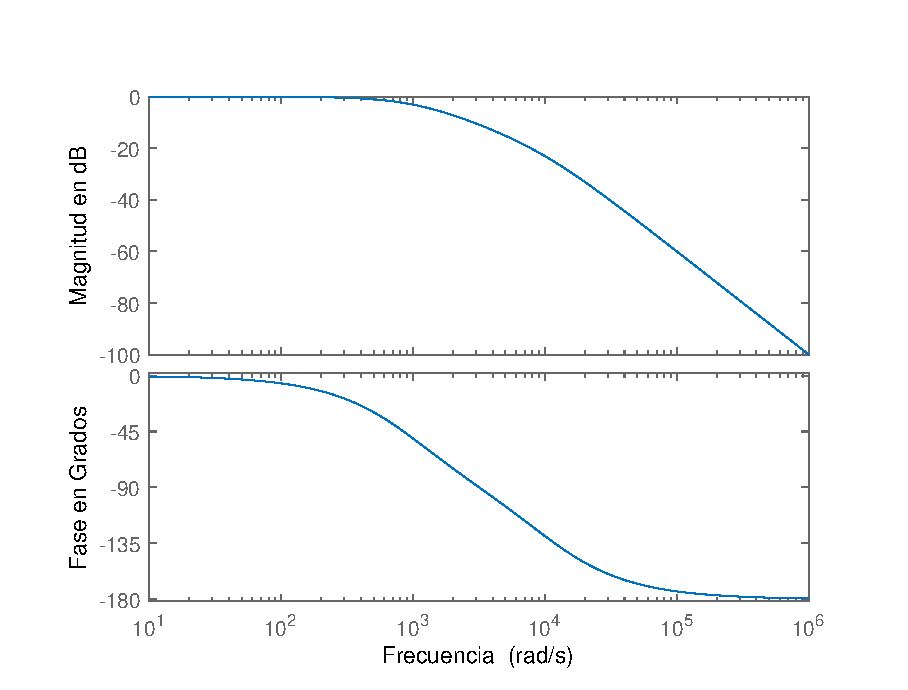
\includegraphics[scale=0.6]{bode}
	\caption{Diagrama de Bode}
\end{center}
\end{figure}

Del análisis del circuito se puede concluir que se trata de un sistema de segundo orden y mediante el Diagrama de Bode confirmar que es un filtro pasabajos.
%Se concluye a partir de la función de transferencia y el diagrama de bode que el circuito presentado conforma un sistema de segundo orden y que el mismo es un filtro pasabajos.

%Por último se obtuvo otro diagrama de bode esta vez simulando el sistema mediante el programa Lt Spice. 
%\begin{figure}[H]
%	\begin{center}
%		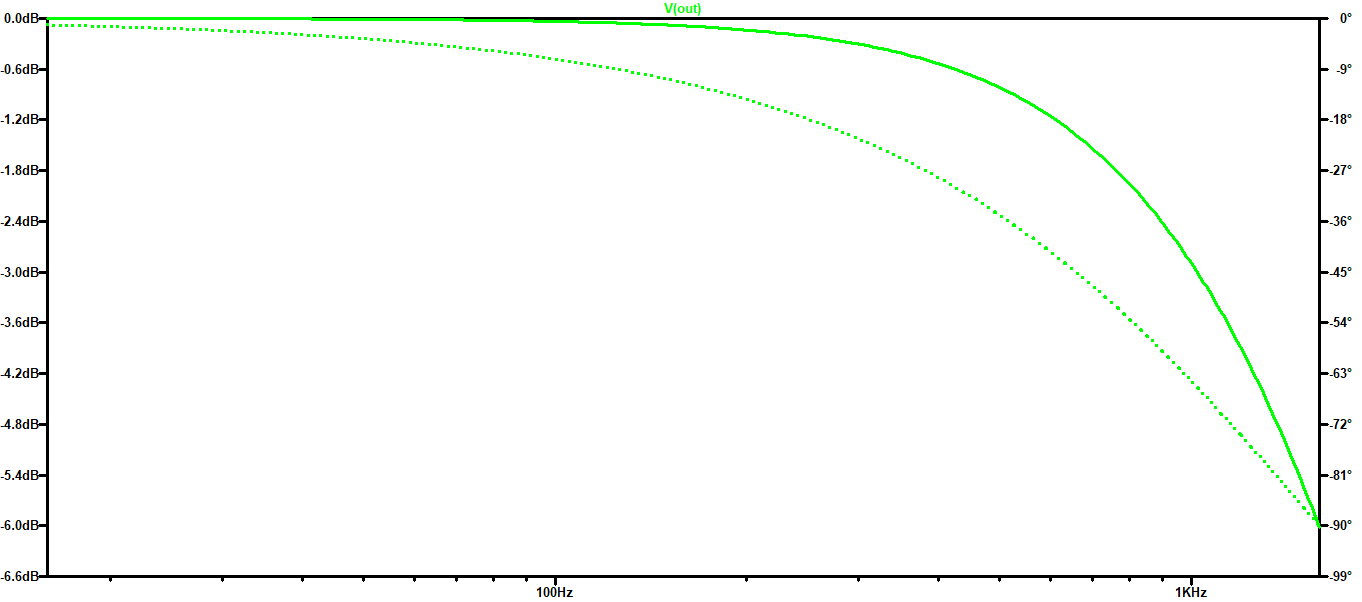
\includegraphics[scale=0.4]{bode3}
%		\caption{Amplitud(Línea continua) y Fase(Linea puntuada)}
%	\end{center}
%\end{figure}
\section{Respuesta en Frecuencia}

Para verificar el comportamiento del circuito se implementó en una protoboard utilizando un Amplificador Operacional TL082 y se realizó un barrido en frecuencia de la señal de entrada con el objetivo de obtener en forma experimental un diagrama de magnitud y fase. Se utilizó un osciloscopio RIGOL DS1052E para medir la salida del circuito y exportar digitalmente las mediciones en formato CSV para luego procesarlo utilizando MATLAB. El formato de los archivos permite representar vectorialmente cada canal y el tiempo en el cual fue adquirida cada muestra.

\begin{figure}[H]
	\begin{center}
		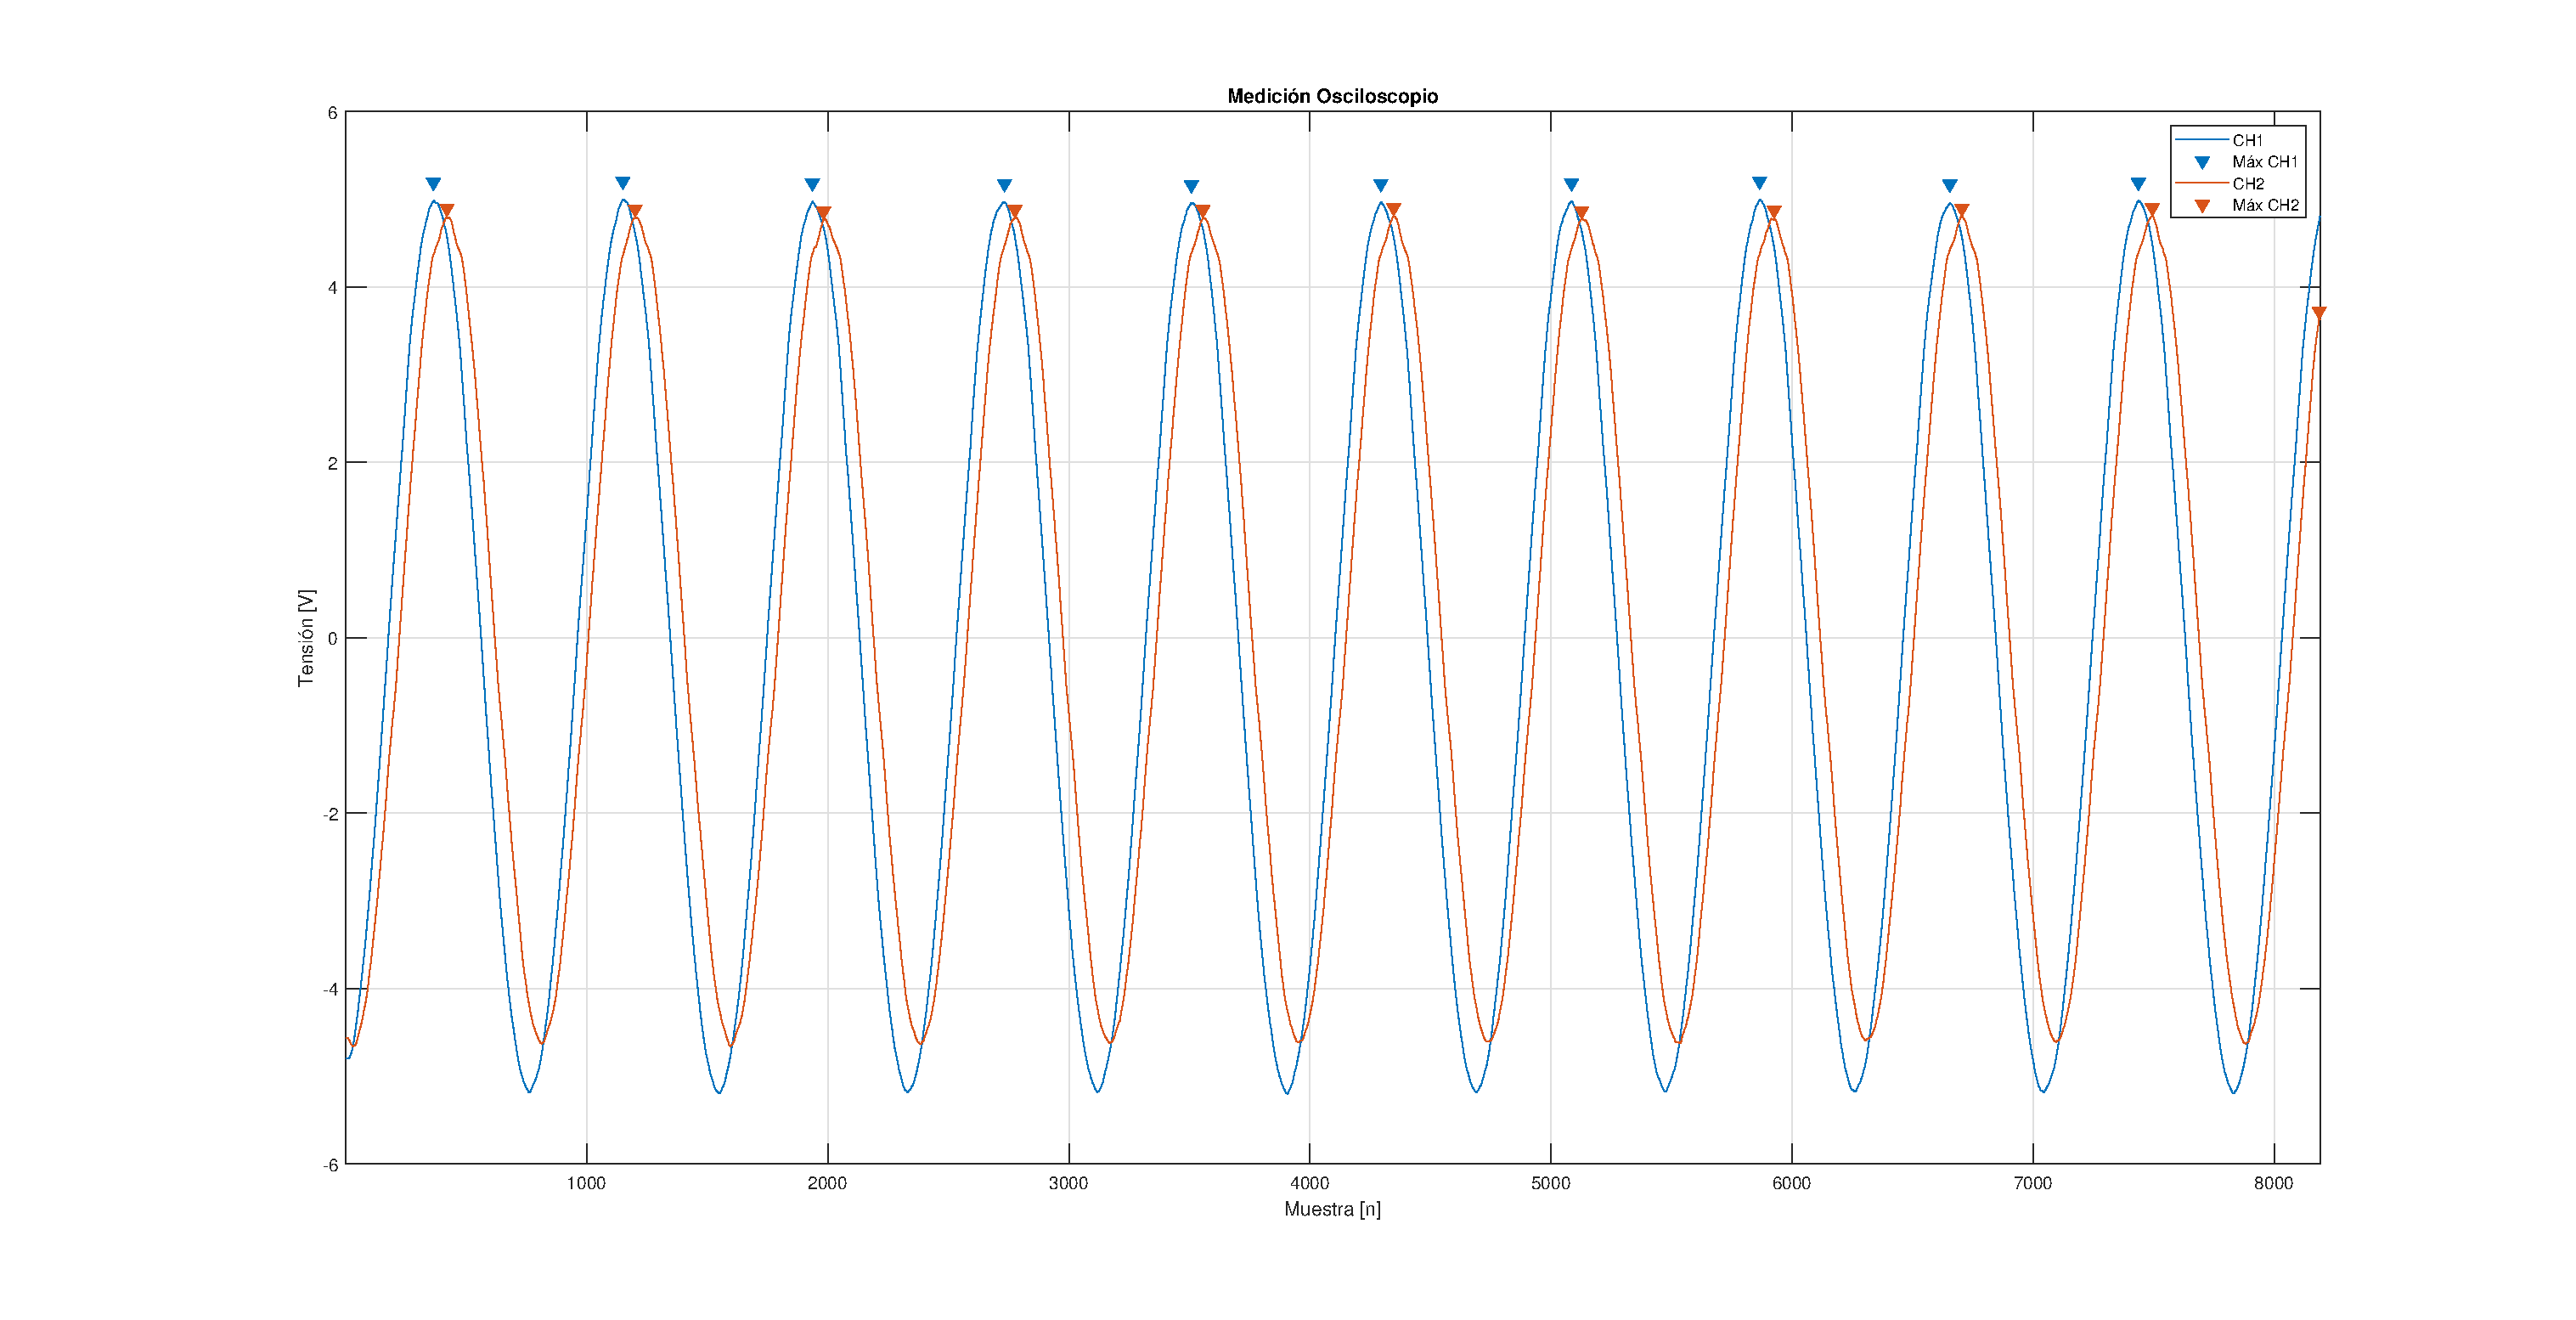
\includegraphics[scale=0.3]{osciloscopio}
		\caption{Frecuencia 400 radianes}
	\end{center}
\end{figure}

Para realizar el Diagrama de Bode se necesitan varios puntos por década, se consideraron los puntos 1, 2 , 3, 4 y 7 de cada década, desde 100 Radianes/s hasta 10k Radianes/s. El script analiza los máximos de cada par de señales y calcula el desfasaje y la ganancia respecto de la señal de referencia, la salida del script son vectores los cuales son representados en una escala semilogaritmica para tener el Diagrama de Bode.

\begin{center}
\begin{tabular}{|c|c|c|}
	\hline 
	Frecuencia & Magnitud & Fase
	\\ 
	\hline 
	100 & 0,259191362 & 6,305732484
	\\ 
	\hline 
	200 & -0,163323083
	& 12,38216561
	\\ 
	\hline 
	300 & -0,188826858
	& 14,77099237
	\\ 
	\hline 
	400 & -0,313267461
	& 22,90076336
	\\ 
	\hline 
	700 & -1,119635495
	& 38,48552339
	\\ 
	\hline 
	2000 & -6,946829452
	& 73,28653478
	\\ 
	\hline 
	3000 & -10,2860529
	& 88,45124283
	\\ 
	\hline 
	4000 & -13,15738713
	& 94,76099426
	\\ 
	\hline 
	7000 & -18,70924479
	& 117,8619154
	\\ 
	\hline 
	10000 & -23,01491137
	& 129,7607656
	\\ 
	\hline 
	20000 & -33,04149488
	& 149,1560102
	\\ 
	\hline 
	30000 & -39,0498078
	& 162,4137931
	\\ 
	\hline 
	40000 & -44,19764534
	& 166,9299363
	\\ 
	\hline 
	70000 & -55,97526234
	& 168,7750557
	\\ 
	\hline 
	100000 & -58,80464233
	& 173,1319555
	\\ 
	\hline 
\end{tabular}   
\end{center} 

%Se implementó el sistema en un protoboard con un generador de funciones y un osciloscopio digital para visualizar la salida y la entrada. Para poder realizar un barrido de frecuencia se vario la frecuencia de la entrada y se tomo los datos de la tensión de la entrada y salida. 
%Para cada frecuencia se guardo un archivo .csv en un pendrive y se realizó un script en matlab para obtener un diagrama de bode con los datos medidos.

Comparando la respuesta experimental con la respuesta ideal:
\begin{figure}[H]
\begin{center}
	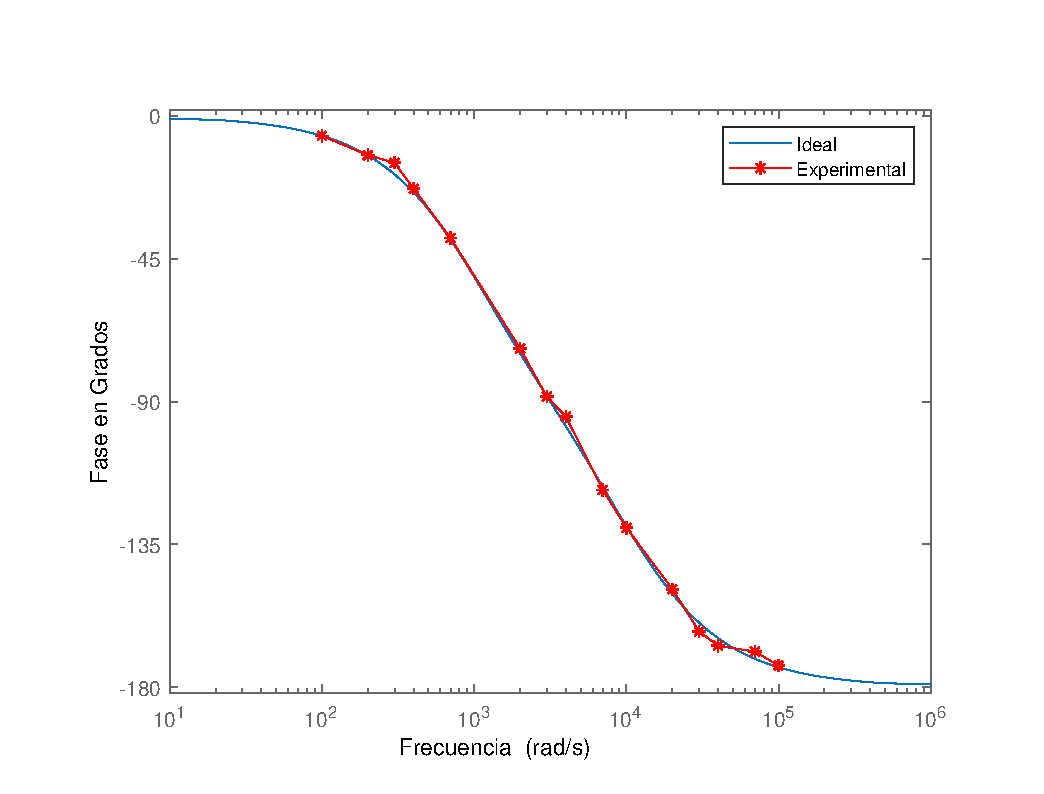
\includegraphics[scale=0.4]{compmag}
	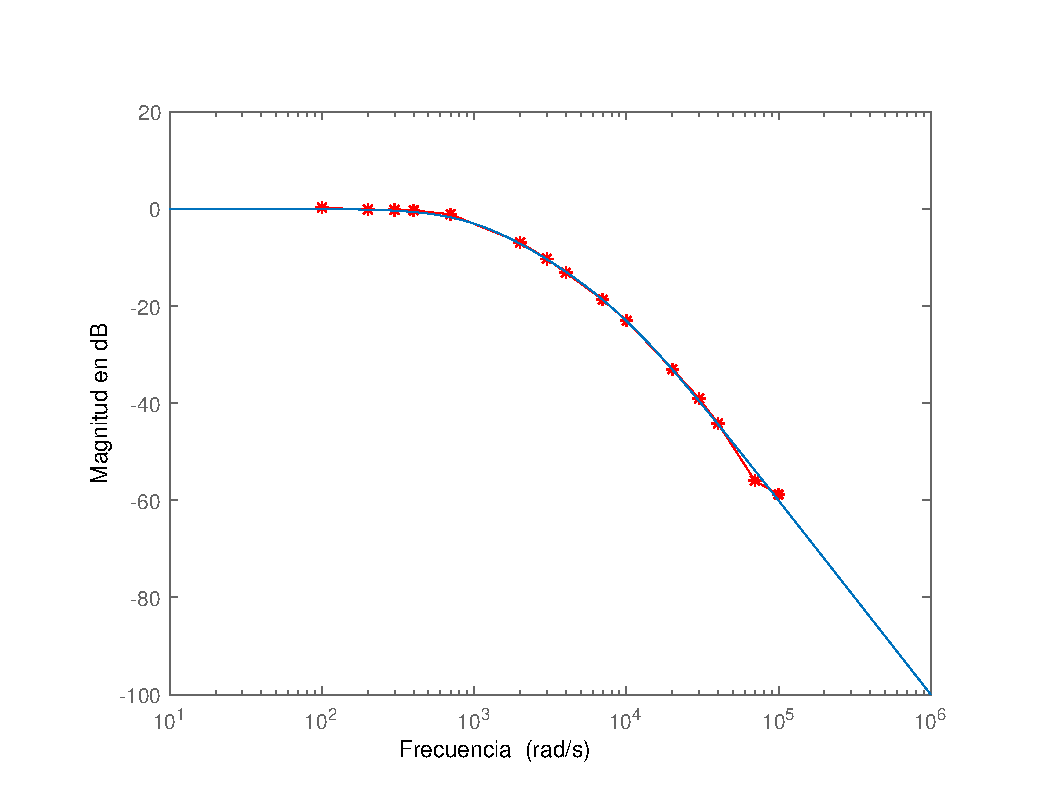
\includegraphics[scale=0.4]{compfase}
	\caption{Comparación diagramas}
\end{center}
\end{figure}

Se observa que el circuito implementado responde como se esperaba en las simulaciones y que el barrido en frecuencia debería ser mas amplio, al menos 2 décadas antes y después de las singularidades del sistema.

\section{Respuesta al escalón}

Para obtener la respuesta al escalón se cambió la forma de onda del generador de funciones a una onda cuadrada de una frecuencia de 100Hz y se exportó la medición a un archivo CSV nuevamente.

\begin{figure}[H]
	\begin{center}
		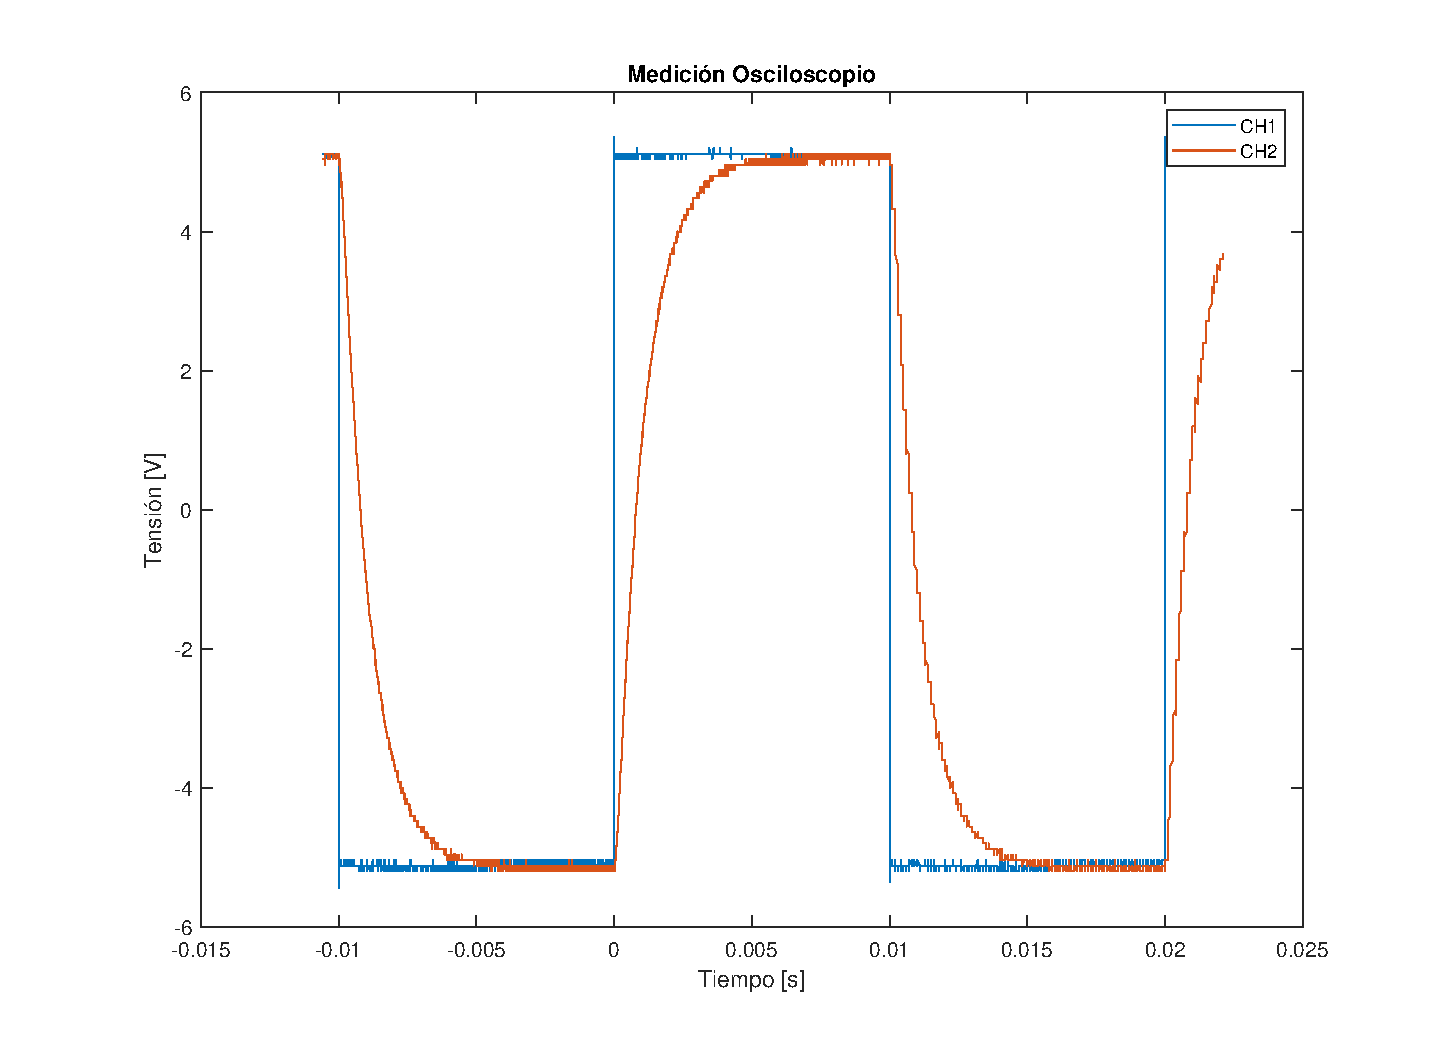
\includegraphics[scale=0.4]{escalonmedido}
		\caption{Respuesta al escalón}
	\end{center}
\end{figure}

Al tratarse de una respuesta sobreamortiguada es posible aproximar la respuesta al escalón con una función exponencial y entonces representar el sistema como uno de primer orden. Esto se debe a que el polo dominante del sistema, es decir el que gobierna la dinámica, está lo suficientemente lejos del otro polo del sistema.
Se puede aproximar la función de transferencia encontrando el valor máximo alcanzado $V_{MAX}$ y una constante de tiempo que queda determinada por el tiempo que tarda el sistema en alcanzar $0.632V_{MAX}$. Hay que tener en cuenta que $V_{MAX}$ en este caso será 10V, pero la función de transferencia debería tener ganancia unitaria según el análisis circuital y en esta aproximación se debe considerar como la proporcion entre la señal de entrada y la salida.
Con un script de MATLAB se encontraron estos valores y la función de transferencia quedó expresada de la siguiente forma:
\begin{equation}
	H(s)=\frac{1}{\tau s + 1}
\end{equation}
Los valores obtenidos:
\begin{center}
	\begin{tabular}{|c|c|}
	\hline 
	Tau & 0.001092 \\ 
	\hline 
	Vmax & 10 \\ 
	\hline 
\end{tabular}
\end{center}
Para poder comparar directamente la función de transferencia aproximada con la medición se expresó la transferencia de la siguiente manera:
\begin{equation}
	H(s)=\frac{10}{0.001092 s + 1}
\end{equation}
 y se obtuvo el siguiente gráfico:
 \begin{figure}[H]
 	\begin{center}
 		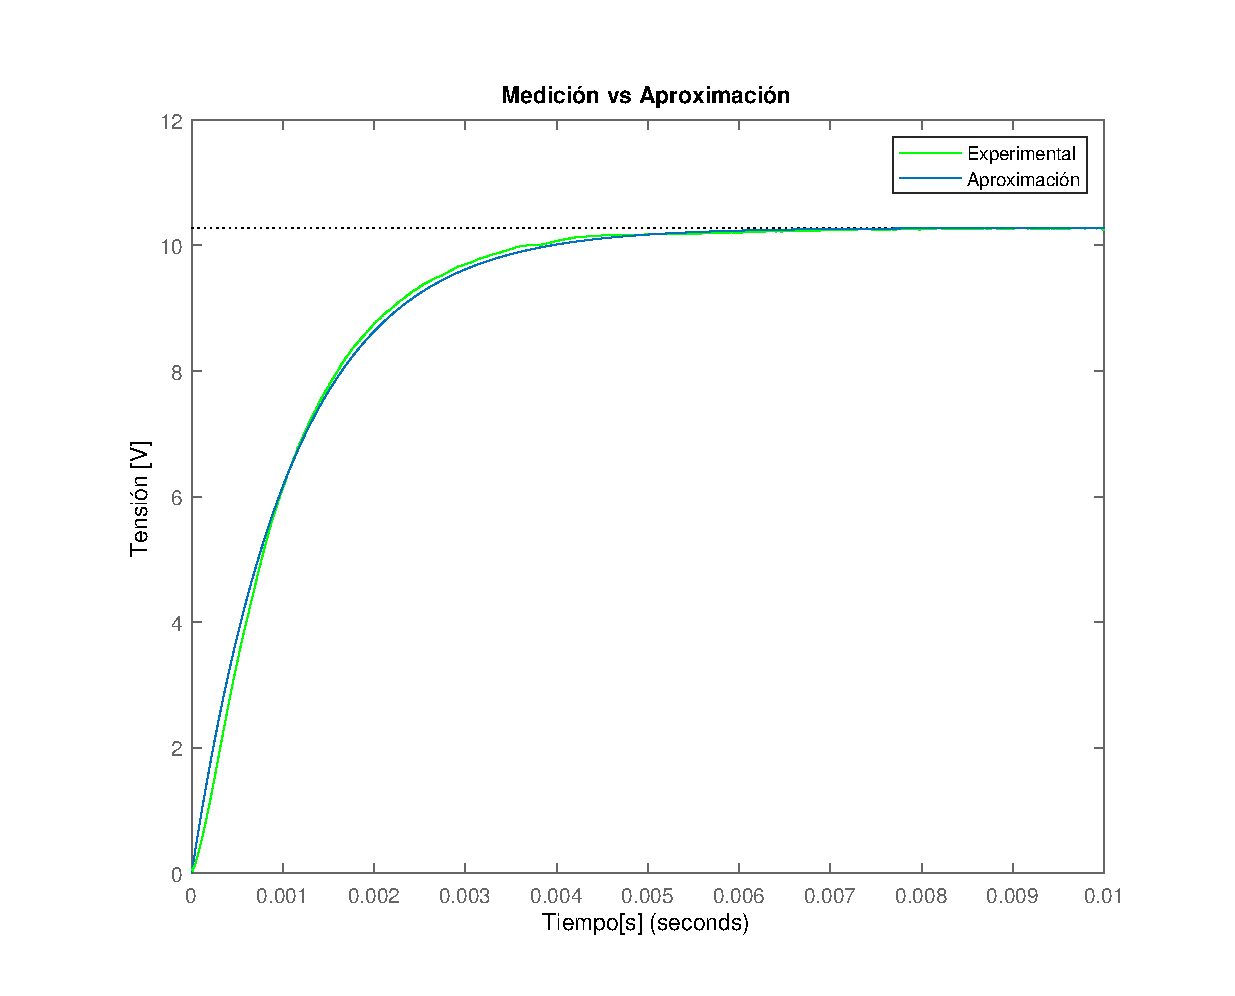
\includegraphics[scale=0.5]{comp1}
 		\caption{Respuestas de los sistemas}
 	\end{center}
 \end{figure}

Se realizó otra comparación, la respuesta del sistema aproximado y la respuesta del sistema ideal:
<<<<<<< HEAD

 \begin{figure}[H]
	\begin{center}
		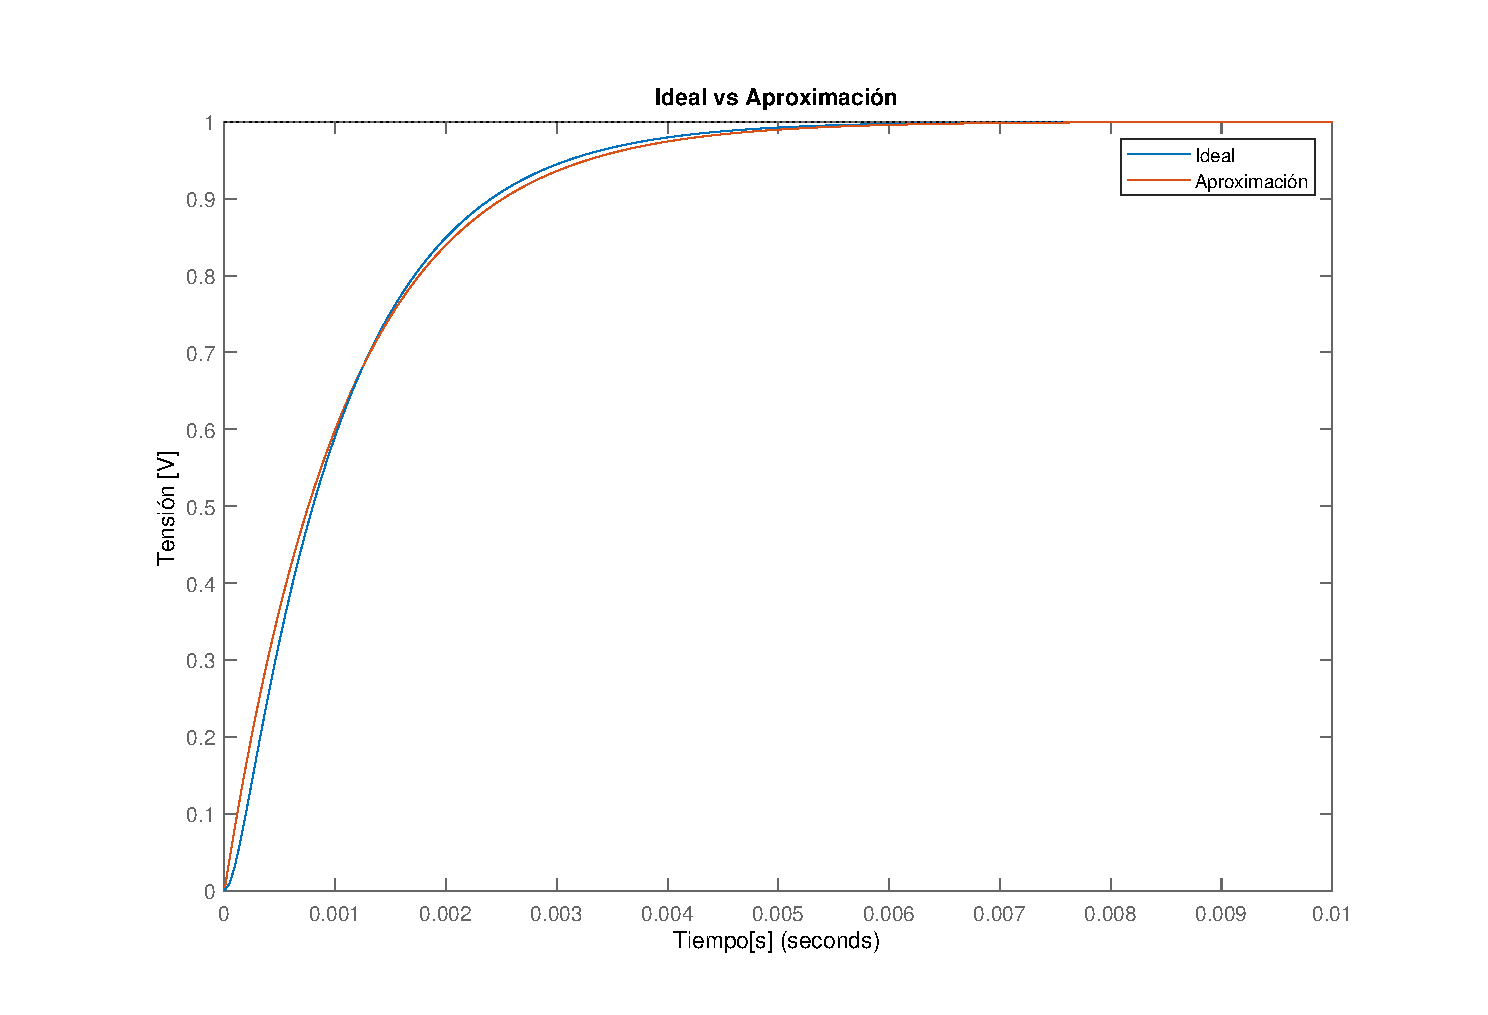
\includegraphics[scale=0.5]{comp2}
		\caption{Respuestas de los sistemas}
	\end{center}
\end{figure}
=======

 \begin{figure}[H]
	\begin{center}
		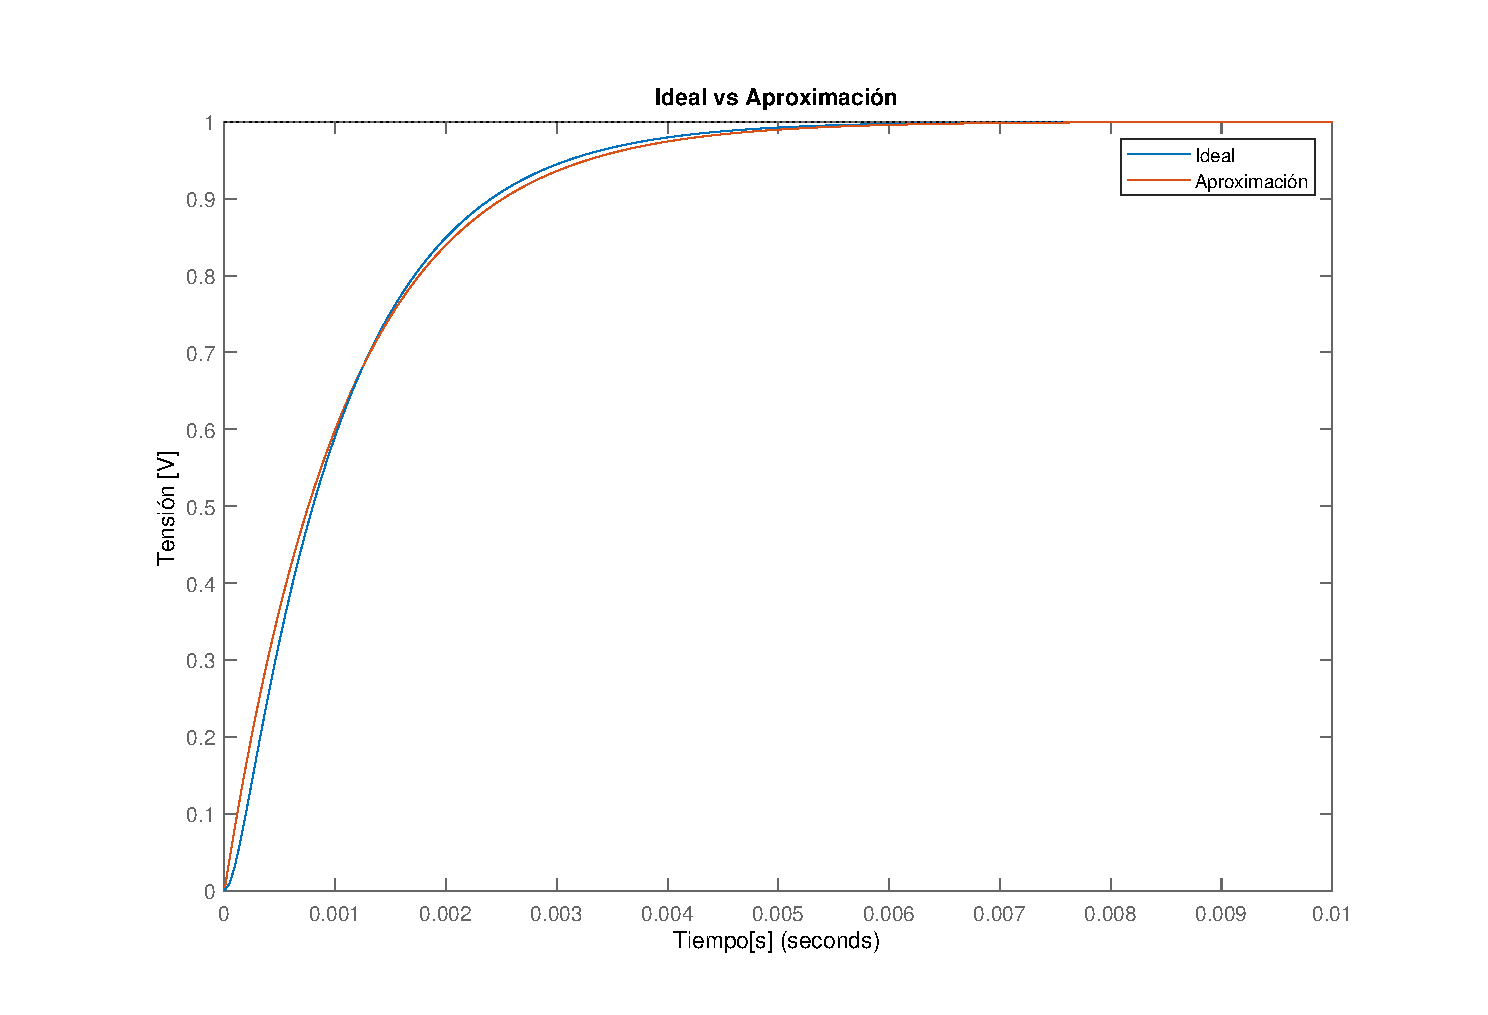
\includegraphics[scale=0.5]{comp2}
		\caption{Respuestas de los sistemas}
	\end{center}
\end{figure}

Se puede observar que las respuestas son similares y por lo tanto la aproximación es buena y puede ser útil para simplificar cálculos.
 
\section{Conclusión}

%vicky la escribe
>>>>>>> 9c16d57984c605e1155575f88475a2047f162bbc

Se puede observar que las respuestas son similares y por lo tanto la aproximación es buena y puede ser útil para simplificar cálculos.
 
\section{Conclusión}
Con los datos medidos de la salida del circuito implementado se generaron los gráficos de bode, los cuales fueron comparados con los obtenidos en el modelo matemático. Se concluye que como los gráficos son similares, el modelo matemático se corresponde con el implementado.

\end{document} 
